Also known as the adjoint state method, it is another example of a discrete method that aims to find the gradient by solving an alternative system of linear equations, known as the \textit{adjoint equations}, at the same time that the original system of linear equations defined by the numerical solver is solved. 
These methods are extremely popular in optimal control theory in fluid dynamics, for example for the design of geometries for vehicles and airplanes that optimize performance \cite{Elliott_Peraire_1996, Giles_Pierce_2000}.

% Mathematically, reverse mode AD is related to the adjoint differential equations \cite{Griewack-on-AD}

\paragraph{Discrete differential equation}

% reference: Sensitivity theory of non-linear systems

The derivation of the discrete adjoint equations is carried once the numerical scheme for solving Equation \eqref{eq:original_ODE} has been specified.  
Given a discrete sequence of timesteps $t_0, t_1, \ldots, t_N$, we evaluate the solution at $u_i = u(t_i; \theta)$. 
Some of the most common numerical solvers include multistep linear solvers of the form 
\begin{equation}
    \sum_{i=0}^{K_1} \alpha_{ni} u_{n-i} 
    +
    h_n \sum_{i=0}^{K_2} \beta_{ni} f(u_{n-i}, \theta, t_{n-i})
    = 
    0.
\end{equation}
and Runge-Kutta methods with 
\begin{align}
    u_{n+1} 
    &= 
    u_n 
    + 
    h \sum_{i=1}^s b_i k_i \\
    k_i 
    &= 
    f \left(u_n + \sum_{j=1}^s a_{ij} k_j , \theta ,  t_n + c_n h \right) \qquad i=1,2, \ldots, s.
\end{align}
The former is linear in $f$, which for example is not the case in Runge-Kutta methods with intermediate evaluations \cite{ascher2008numerical}.
Explicit methods are characterized by $\beta_{n, 0} = 0$ for the multistep and $a_{ij}=0$ if $i \leq j$ for Runge-Kutta methods, otherwise, the method is implicit. 

For multistep methods, solving the differential equation implies to be able to solve the system of constraints
\begin{equation}
    g_i(u_i; \theta) = u_i - h \beta_{n0} f(u_i, \theta, t_i) - \alpha_i = 0
\end{equation}
where $\alpha_i$ has includes the information of all the past iterations. 
This system can be solved sequentially, by solving for $u_i$ in increasing order of index using Newton method. 
If we call the super-vector $U = (u_1, u_2, \ldots, u_N) \in \R^{nN}$, we can combine all these equations into one single system of equations $G(U) = (g_1(u_1; \theta), \ldots, g_N(u_N; \theta)) = 0$.

In the simplest case of linear one-step methods with $g_i (u_{i+1}; \theta) = u_{i+1} - A_i (\theta) \, u_i - b_i$ with $A_i \in \R^{n \times n}$ and $b_i \in \R^n$ defined by the numerical solver, the condition $G(U)=0$ simplifies to the linear system of equations 
\begin{equation}
    A(\theta) U 
    = 
    \begin{bmatrix}
        \I_{n \times n} & 0 &   &  & \\
        -A_1 & \I_{n \times n} & 0 &  &  \\
          & -A_2 & \I_{n \times n} & 0 &  \\
         &  &   & \ddots &   \\
         &  &  & -A_{N-1} & \I_{n \times n}
    \end{bmatrix}
    \begin{bmatrix}
        u_1 \\
        u_2 \\
        u_3 \\
        \vdots \\
        u_N
    \end{bmatrix}
    = 
    \begin{bmatrix}
        A_0 u_0 + b_0 \\
        b_1 \\
        b_2 \\
        \vdots \\
        b_{N-1}
    \end{bmatrix}
    = 
    b(\theta), 
\end{equation}
with $\I_{n \times n}$ the identity matrix of size $n \times n$.
% It is usually convenient to write this system of linear equations in the residual form $G(U; \theta) = 0$, where $G(U; \theta) = A(\theta) U - b(\theta)$ is the residual between both sides of the equation. 
% Different numerical schemes will lead to different design matrix $A(\theta)$ and vector $b(\theta)$, but ultimately every numerical method will lead to a system of linear equations with the form $G(U; \theta) = A(\theta) U - b(\theta) = 0$ after being discretized. 
It is important to notice that in most cases, the matrix $A(\theta)$ is quite large and mostly sparse. 
If this representation of the discrete differential equation is quite convenient for mathematical manipulations, at the moment of solving the system we will rely in iterative solvers that save memory and computation. 

\paragraph{Adjoint state equations}

We are interested in differentiating a function $L(U, \theta)$ with respect to the parameter $\theta$. 
Since here $U$ is the discrete set of evaluations of the solution, examples of loss functions now include 
\begin{equation}
    L(U, \theta) 
    = 
    \frac{1}{2} \sum_{i=1}^N \| u_i - u_i^\text{obs} \|^2, 
\end{equation}
with $u_i^\text{obs}$ the observed time-series. 
We further need to impose the constraint that the solution satisfies the algebraic linear equation $G(U; \theta) = 0$.
Now,
\begin{equation}
    \frac{dL}{d\theta} 
    = 
    \frac{\partial L}{\partial \theta} 
    + 
    \frac{\partial L}{\partial U} \frac{\partial U}{\partial \theta},
    \label{eq:dhdtheta0}
\end{equation}
and also for the constraint $G(U; \theta)=0$ we can derive
\begin{equation}
    \frac{dG}{d\theta} 
    = 
    \frac{\partial G}{\partial \theta} 
    + 
    \frac{\partial G}{\partial U} \frac{\partial U}{\partial \theta}
    =
    0
\end{equation}
which is equivalent to 
\begin{equation}
    \frac{\partial U}{\partial \theta} 
    = 
    - \left( \frac{\partial G}{\partial U} \right)^{-1} \frac{\partial G}{\partial \theta}.
\end{equation}
If we replace this last expression into equation \eqref{eq:dhdtheta0}, we obtain
\begin{equation}
    \frac{dL}{d\theta} 
    =
    \frac{\partial L}{\partial \theta} 
    - 
    \underbrace{\frac{\partial L}{\partial U}}_{\text{vector}}
    \left( \frac{\partial G}{\partial U} \right)^{-1} 
    \frac{\partial G}{\partial \theta}.
    \label{eq:dhdtheta}
\end{equation}
The important trick in the adjoint state methods is to observe that in this last equation, the right-hand side can be resolved as a vector-Jacobian product (VJP).
Instead of computing the product of the matrices $\left( \frac{\partial G}{\partial U} \right)^{-1}$ and $\frac{\partial G}{\partial \theta}$, it is computationally more efficient first to compute the resulting vector from the operation $\frac{\partial L}{\partial U} \left( \frac{\partial G}{\partial U} \right)^{-1}$ and then multiply this by $\frac{\partial G}{\partial \theta}$.
This is what leads to the definition of the adjoint $\lambda \in \R^{nN}$ as the solution of the linear system of equations 
\begin{equation}
    \left( \frac{\partial G}{\partial U}\right)^T \lambda 
    =  
    \left( \frac{\partial L}{\partial U} \right)^T,
    \label{eq:adjoint-state-equation}
\end{equation}
that is,
\begin{equation}
    \lambda^T = \frac{\partial L}{\partial U} \left( \frac{\partial G}{\partial U} \right)^{-1}.
    \label{eq:def_adjoint}
\end{equation}
Finally, if we replace Equation \eqref{eq:def_adjoint} into \eqref{eq:dhdtheta}, we obtain 
\begin{equation}
    \frac{dL}{d\theta} 
    =
    \frac{\partial L}{\partial \theta} 
    - 
    \lambda^T \frac{\partial G}{\partial \theta}.
    \label{eq:gradient-adjoint-state-method}
\end{equation}
The important trick to notice here is the rearrangement of the multiplicative terms involved in equation \eqref{eq:dhdtheta}. 
Computing the full Jacobian/sensitivity $\partial U / \partial \theta$ will be computationally expensive and involves the product of two matrices. 
However, we are not interested in the calculation of the Jacobian, but instead in the VJP given by $\frac{\partial L}{\partial U} \frac{\partial U}{\partial \theta}$. 
By rearranging these terms and relying in the intermediate variable $G(U; \theta)$, we can make the same computation more efficient. 
These ideas are summarized in the diagram in Figure \ref{fig:discrete-adjoint}, where we can also see an interesting interpretation of the adjoint as being equivalent to $\lambda^T = - \frac{\partial L}{\partial G}$. 

\begin{figure}[t]
    \centering
    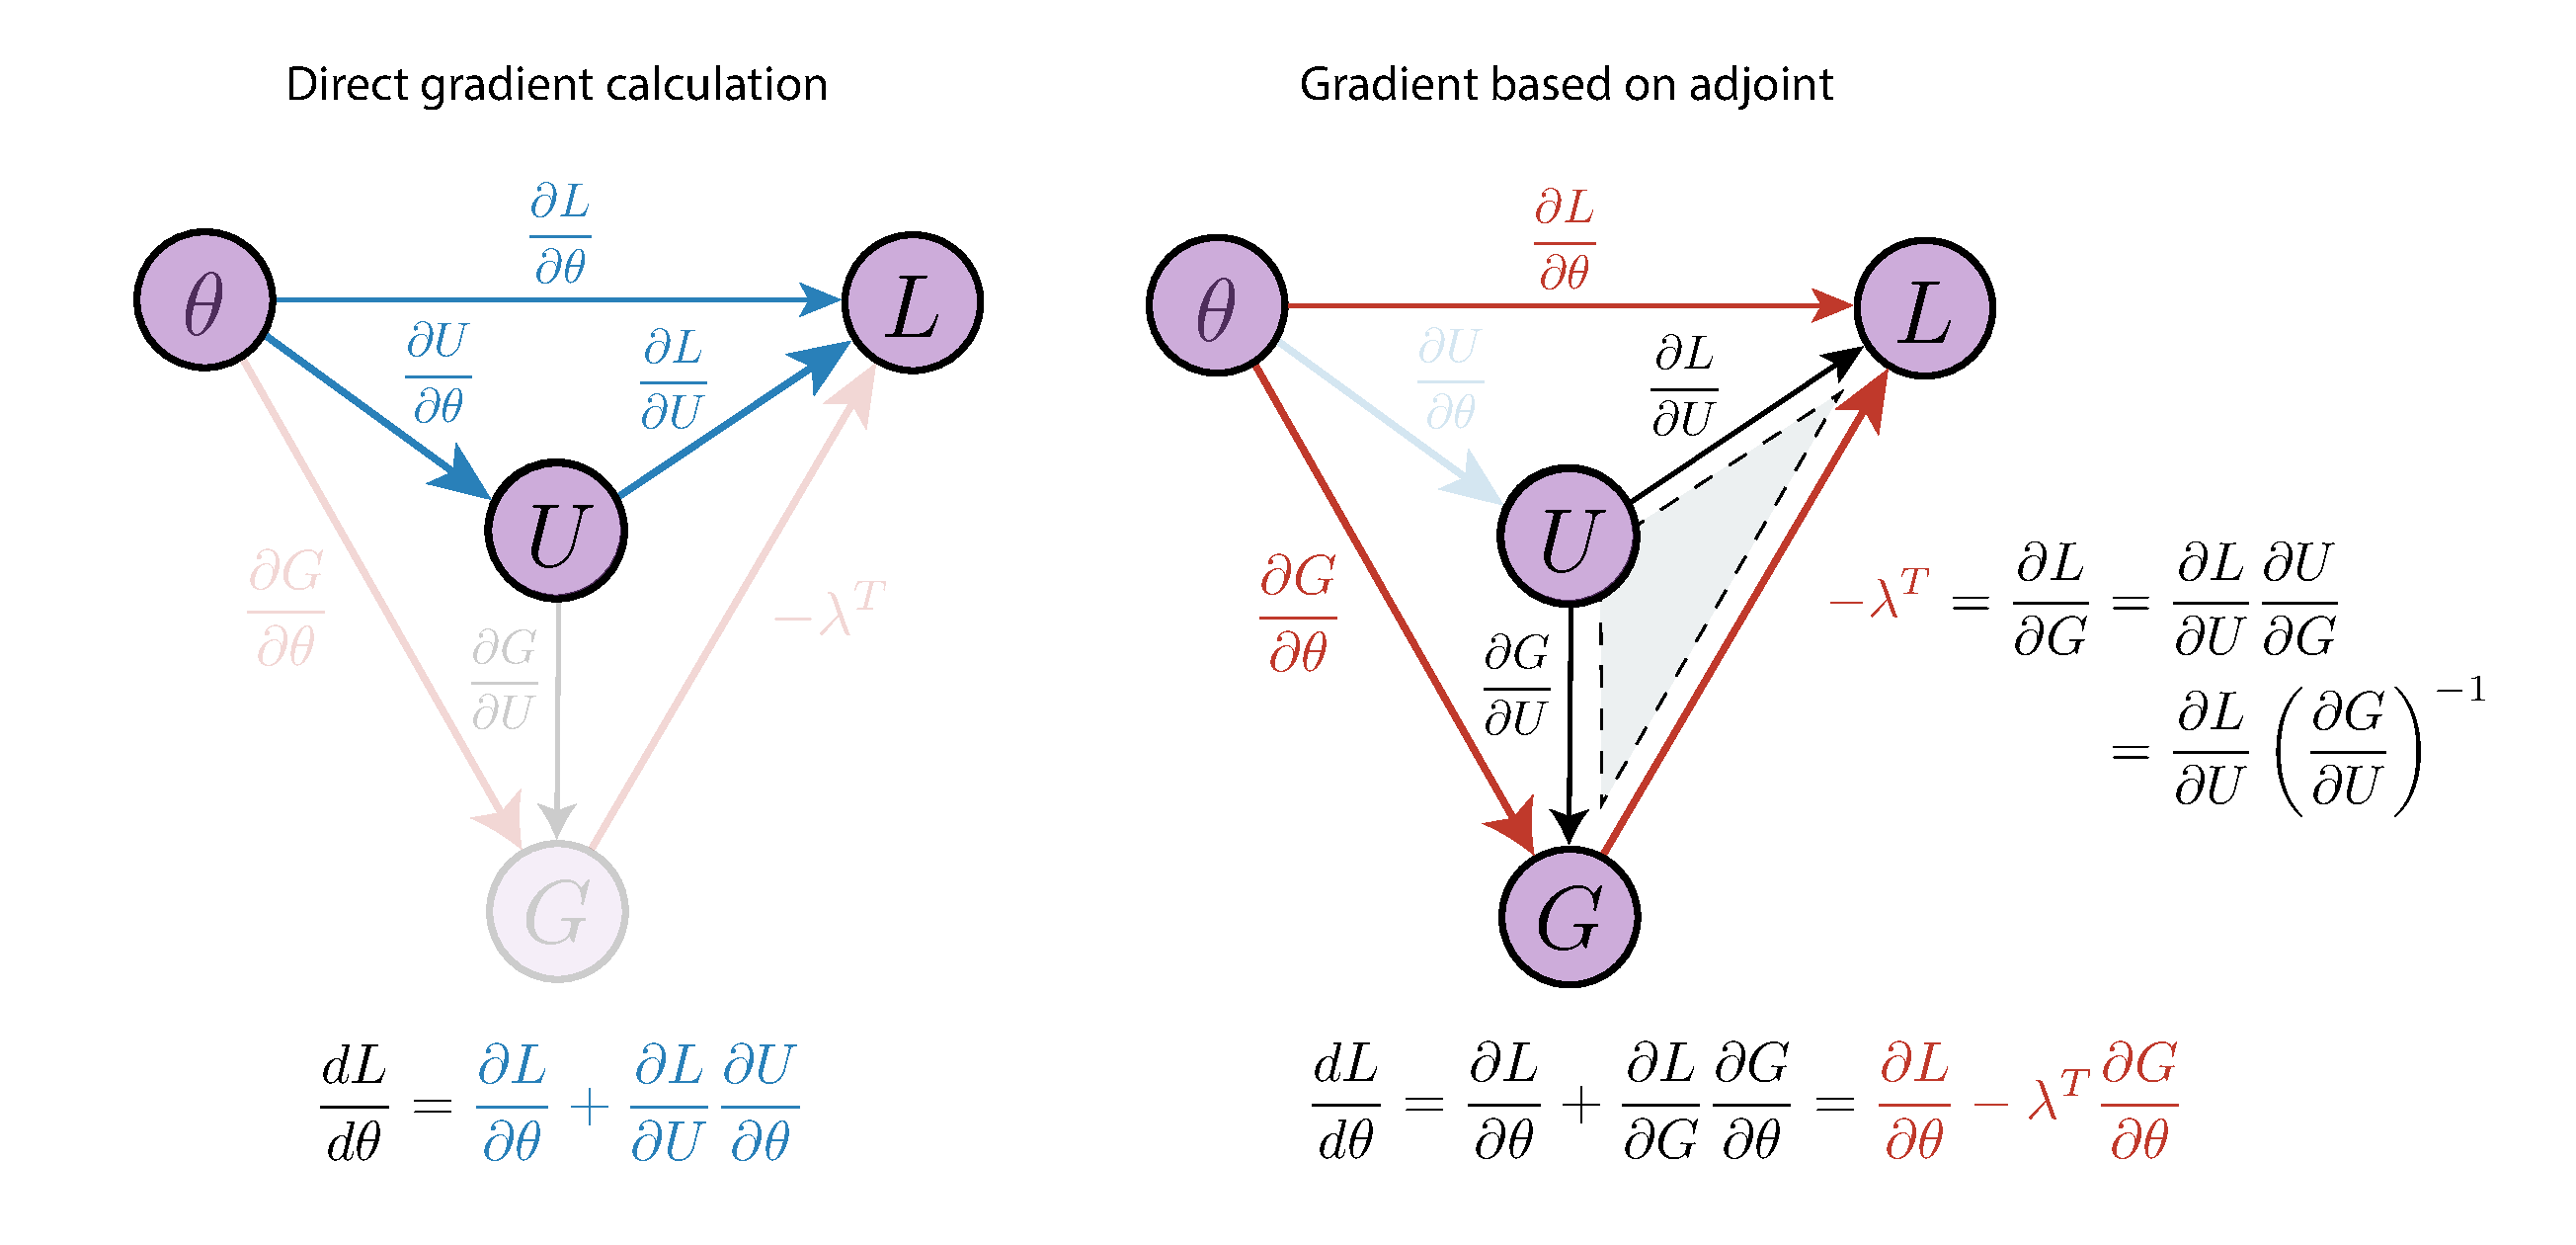
\includegraphics[width=0.95\textwidth]{figures/discrete_adjoint.pdf}
    \caption{Diagram showing how gradients are computed using discrete adjoints. On the left, we see how gradients will be computed if we use the chain rule applied to the directed triangle defined by the variables $\theta$, $U$, and $L$ (blue arrows). However, we can define the intermediate variable $G(U; \theta) = 0$ (defined by the discrete system of differential equations) and apply the chain rule instead to the triangle defined by $\theta$, $G$, and $L$ (red arrows). In the red diagram, the calculation of $\frac{\partial L}{\partial G}$ is done by pivoting in $U$ as its is shown in the right diagram (shaded area). Notice that the use of adjoints avoids the calculation of the sensitivity $\frac{\partial U}{\partial \theta}$. The adjoint is defined as the partial derivative $\lambda^T = - \frac{\partial L}{\partial G}$ representing changes in the lost function due to variations in the discrete equation $G(U; \theta) = 0$. 
    }
    \label{fig:discrete-adjoint}
\end{figure}

Notice that the algebraic equation of the adjoint $\lambda$ in Equation \eqref{eq:adjoint-state-equation} is a linear system of equations even when the original system $G(U)=0$ was not necessarily linear in $U$.
This means that while the forward mode may required multiple iterations calls in order to solve the non-linear system $G(U) = 0$ using Krylov methods, the backwards step to compute the adjoint is one single linear system of equations. 
For the linear system of discrete equations $G(U; \theta)=A(\theta) U - b(\theta)=0$, we have \cite{Johnson}
\begin{equation}
    \frac{\partial G}{\partial \theta} 
    = 
    \frac{\partial A }{\partial \theta} U - \frac{\partial b}{\partial \theta},
\end{equation}
so the desired gradient in Equation \eqref{eq:gradient-adjoint-state-method} can be computed as 
\begin{equation}
    \frac{dL}{d\theta} 
    = 
    \frac{\partial L}{\partial \theta} 
    - 
    \lambda^T \left( \frac{\partial A }{\partial \theta} U - \frac{\partial b}{\partial \theta} \right)
    \label{eq:dhdtheta_linear}
\end{equation}
with $\lambda$ the solution of the linear system (Equation \eqref{eq:adjoint-state-equation})
\begin{equation}
    A(\theta)^T \lambda 
    =
    \begin{bmatrix}
        \I_{n \times n} & -A_1^T &   &  & \\
        0 & \I_{n \times n} & -A_2^T &  &  \\
          & 0 & \I_{n \times n} & -A_3^T &  \\
         &  &   & \ddots & -A_{N-1}^T  \\
         &  &  & 0 & \I_{n \times n}
    \end{bmatrix}
    \begin{bmatrix}
        \lambda_1 \\
        \lambda_2 \\
        \lambda_3 \\
        \vdots \\
        \lambda_N
    \end{bmatrix}
    = 
    \begin{bmatrix}
        u_1 - u_1^\text{obs} \\
        u_2 - u_2^\text{obs} \\
        u_3 - u_3^\text{obs} \\
        \vdots \\
        u_N - u_N^\text{obs}     
    \end{bmatrix}
    = 
    \frac{\partial L}{\partial U}^T.
    \label{eq:linea-adjoint-state-equation}
\end{equation}
This is a linear system of equations with the same size of the original $A(\theta) U = b(\theta)$, but involving the adjoint matrix $A^T$. 
Computationally this also means that if we can solve the original system of discretized equations then we can also solve the adjoint. 
One way of doing this is relying on matrix factorization. 
Using the LU factorization we can write the matrix $A(\theta)$ as the product of a lower and upper triangular matrices $A (\theta) = LU$, which then can be also used for solving the adjoint equation since $A^T(\theta)=U^TL^T$.
Another more natural way of finding the adjoints $\lambda$ is by noticing that the system of equations \eqref{eq:linea-adjoint-state-equation} is equivalent to the iterative scheme
\begin{equation}
    \lambda_{i} = A_{i}^T \lambda_{i+1} + (u_i - u_i^\text{obs})
\end{equation}
with initial condition $\lambda_N$. 
This means that we can solve the adjoint equation in backwards mode, starting from the final state $\lambda_N$ and computing the values of $\lambda_i$ in decreasing index order. 
Notice that this procedure requires to know the value of $u_i$ at any given timestep. 
% When do we solve this backwards and when forward?


%In order to compute the gradient of the full solution of the differential equation, we apply this method sequentially using the chain rule. One single step of the state method can be understood as the chain of operations $\theta \mapsto g \mapsto u \mapsto L$. This allows us to create adjoints for any primitive function $g$ (i.e. the numerical solver scheme) we want, and then incorporated it as a unit of any AD program. 

% \subsubsection{Further remarks}

% Conection with duality
% Conection with the adjoint operator
% Different ways of deriving the adjoint equations: lagrangian
% Is the adjoint the same than a gradient? Yes, but these are derivatives with respect to the state of the system, not with respect to the parameters! 